\documentclass{llncs}
\usepackage{placeins}
\usepackage[T1]{fontenc}
\usepackage{pdflscape}
\usepackage{newtxtext}
\usepackage[varvw]{newtxmath}
\usepackage{float}
\usepackage{graphicx}
\usepackage{amsmath}
\usepackage{booktabs}
\usepackage{multirow}
\usepackage{tabularx}
\usepackage{array}
\usepackage{makecell}

\graphicspath{{figures/}}

\setlength{\emergencystretch}{3em}
\begin{document}

\title{Target-Conditioned Evidence Retrieval for Knowledge Tracing}
\author{}
\maketitle

\begin{abstract}
Knowledge tracing predicts student responses from their learning histories to support personalized learning. As intelligent tutoring systems (ITS) expand their question banks, they must predict responses to questions involving new knowledge components (KCs). Historical responses can inform these predictions through shared concepts, cognitive demands, and structural relations. Evidence selection therefore needs to consider both target relevance and complementary information. We propose Cognitive-RAG KT, a target-conditioned evidence retrieval framework. It recalls candidate interactions through multiple relations and selects a complementary evidence set by balancing target relevance, relation coverage, and redundancy. Structured relation attributes and a schema-constrained summary organize the selected responses into a prediction context. This context and the target-question representation are projected into continuous soft slots of a frozen language model to predict the probability of a correct response. Experiments on three public datasets show that Cognitive-RAG KT outperforms the evaluated KT baselines.

\keywords{
Knowledge Tracing \and Educational Data Mining \and Large Language Models
}

\end{abstract}

\section{Introduction}

Intelligent tutoring systems (ITS) support personalized practice and learning assistance. Knowledge tracing (KT) uses students' learning histories to predict whether they will answer questions correctly, providing a basis for these services. As question banks expand, students encounter questions involving new knowledge components. Predicting responses to these questions requires connecting the demands of new content with students' performance in previous practice.

Recurrent and memory-based models, including DKT and DKVMN, encode historical responses into an evolving representation of a student's knowledge~\cite{piech2015deep,zhang2017dynamic}. Attention-based methods such as SAKT and AKT assign attention weights to historical interactions according to their relevance to the target question~\cite{pandey2019sakt,ghosh2020akt}. Retrieval-based KT further incorporates selected records into prediction, as illustrated by CoKT's retrieval of response sequences from similar students~\cite{long2022cokt}. For new questions and concepts, inductive approaches use textual descriptions and structural relations to construct representations beyond question and concept identifiers~\cite{fu2024sinkt}. These approaches represent educational content and relate past responses to subsequent performance.

Textual and structural representations provide a basis for connecting questions involving new KCs to previously observed content. We focus on selecting historical responses that jointly inform prediction for such questions. Historical questions may connect to the target through shared concepts, prerequisite knowledge, or similar cognitive demands. Selecting several highly similar questions may repeat information about one requirement while leaving others poorly represented. Evidence selection should therefore account for both the relevance of each interaction and the additional information it contributes to the selected set.

Consider a question that asks for the final bead's color and the number of beads of that color in a repeating arrangement. Answering it involves both locating an element within a cycle and counting occurrences across cycles. Responses to historical position-finding and counting questions reflect performance on these two requirements, respectively. Selecting several position-finding questions may yield repeated information without showing the student's performance on counting. Combining responses from both types provides evidence about both requirements of the target.

To select such evidence, we propose Cognitive-RAG KT, a target-conditioned evidence retrieval framework for predicting responses to questions involving new KCs. Candidate recall uses conceptual, cognitive, graph, and collaborative relations to identify historical interactions connected to the target. Reranking and greedy selection balance target relevance, relation coverage, and redundancy to construct an evidence set. Each selected response retains attributes describing its question's relation to the target. A schema-constrained summary brings these observations together into an account of the student's relevant performance. The evidence context and target-question representation are then projected into soft slots of a frozen language model to predict the probability of a correct response.

This work makes two contributions to predicting student responses on questions involving new KCs. First, we develop a two-stage retrieval strategy that selects complementary historical interactions by balancing target relevance, incremental concept and relation coverage, and redundancy within the evidence set. Second, we construct an evidence context from selected responses, their relations to the target, and a structured summary, and connect it to a frozen language model through soft slots. Experiments on three public datasets show improved prediction performance, while ablation studies assess the contributions of evidence selection and context construction.

\section{Related Work}

\subsection{Modeling Student Interaction Histories}

State-based KT models describe student knowledge through probabilistic transitions or learned representations of response sequences. Bayesian Knowledge Tracing models mastery of each KC as a binary state that evolves through probabilistic transitions~\cite{corbett1995knowledge}. DKT uses a recurrent neural network to learn a sequential representation of student knowledge from past responses~\cite{piech2015deep}. DKVMN organizes concepts in a static key memory and updates student knowledge in a dynamic value memory~\cite{zhang2017dynamic}.

Attention-based KT models weight historical interactions by their relevance to the target question. SAKT identifies relevant past interactions through self-attention to predict a student's response~\cite{pandey2019sakt}. In AKT, attention weights combine question similarity with context-aware distance and exponential decay~\cite{ghosh2020akt}. simpleKT represents differences among questions through question-specific variations and applies ordinary dot-product attention to historical interactions~\cite{liu2023simplekt}. sparseKT retains high-scoring historical interactions through soft-thresholding or top-$K$ sparse attention~\cite{huang2023sparsekt}. DenoiseKT combines graph-enhanced question representations with denoised attention to reduce the influence of irrelevant historical information~\cite{deng2025denoisekt}.

\subsection{Inductive Representations for Questions and Knowledge Components}

Inductive KT uses textual and structural information to represent newly introduced questions and concepts. SINKT encodes question and concept descriptions with a pretrained language model to obtain semantic representations~\cite{fu2024sinkt}. It constructs a heterogeneous graph from question-concept associations and LLM-generated concept relations, then aggregates neighboring representations to incorporate structural information into response prediction.

\subsection{Retrieval and Language Models in Knowledge Tracing}

Retrieval-based KT draws on historical records and structured resources to construct context for prediction. CoKT retrieves response records and sequences from students with similar learning histories and integrates this inter-student information with the target student's history~\cite{long2022cokt}. RAG-KT combines behavioral, structural, and ability-based similarities to retrieve similar students and organizes individual and peer performance into a structured context for cross-platform prediction and interpretable diagnosis~\cite{duan2026ragkt}. Our retrieval selects interactions from the target student's own history, using target relevance together with concept and relation coverage gains and redundancy relative to the selected evidence.

Language-model-based KT combines question semantics with student interaction representations for response prediction. LLM-KT uses plug-in context and sequence components to map textual and behavioral representations into a language model's embedding space~\cite{wang2025llmkt}. Related parameter-efficient adaptation methods use trainable continuous representations to adapt frozen language models to downstream tasks. Prefix tuning learns prefix activations across Transformer layers, whereas prompt tuning prepends trainable embeddings to the model input~\cite{li2021prefixtuning,lester2021power}.

In Cognitive-RAG KT, history soft slots are constructed from selected response records, their relations to the target, and a structured summary. A separate projector maps the target-question representation into target soft slots.

\section{Method}

\subsection{Problem Formulation}

Let $\mathcal U$, $\mathcal Q$, and $\mathcal C$ denote the sets of students, questions, and knowledge concepts (KCs), respectively. Each question $q\in\mathcal Q$ is associated with a concept set $\mathcal C(q)\subseteq\mathcal C$. Let $\mathcal C_{\mathrm{tr}}$ denote the training concepts, which occur in the training response records. The new concepts $\mathcal C_{\mathrm{ho}}$ do not occur in these records, with $\mathcal C_{\mathrm{tr}}\cap\mathcal C_{\mathrm{ho}}=\emptyset$.

For a student $u$, the response history before step $t$ is

\[\mathcal H_t=\left\{(q_i,y_i)\mid 1\leq i<t,\;\mathcal C(q_i)\subseteq\mathcal C_{\mathrm{tr}}\right\},\]

where $q_i$ is the question attempted at step $i$ and $y_i\in\{0,1\}$ is its observed response outcome. Given $\mathcal H_t$ and a target question $q_t$, the model estimates the probability of a correct response:

\[\hat p_t=P(y_t=1\mid\mathcal H_t,q_t).\]

Test targets satisfy $\mathcal C(q_t)\cap\mathcal C_{\mathrm{ho}}\neq\emptyset$.

\subsection{Framework Overview}

Figure~\ref{fig:cognitive-rag-overview} summarizes Cognitive-RAG KT. Given a student's interaction history $\mathcal H_t$ and a target question $q_t$, the framework has four components: question representation, historical interaction retrieval, context construction, and response prediction. First, it represents the target and historical questions using textual, semantic, and collaborative information. Second, it scores historical interactions by their relations to $q_t$, reranks the retained candidates, and selects an evidence set $E_t$ containing up to $K$ interactions from $\mathcal H_t$. Third, it encodes the selected interactions, their response outcomes, and a structured summary into a context representation. Finally, it projects the context and target-question representations into the embedding space of a frozen large language model. The correct response probability $\hat p_t$ is computed from the logits of the correct and incorrect label tokens.

\begin{figure}[t]
\centering
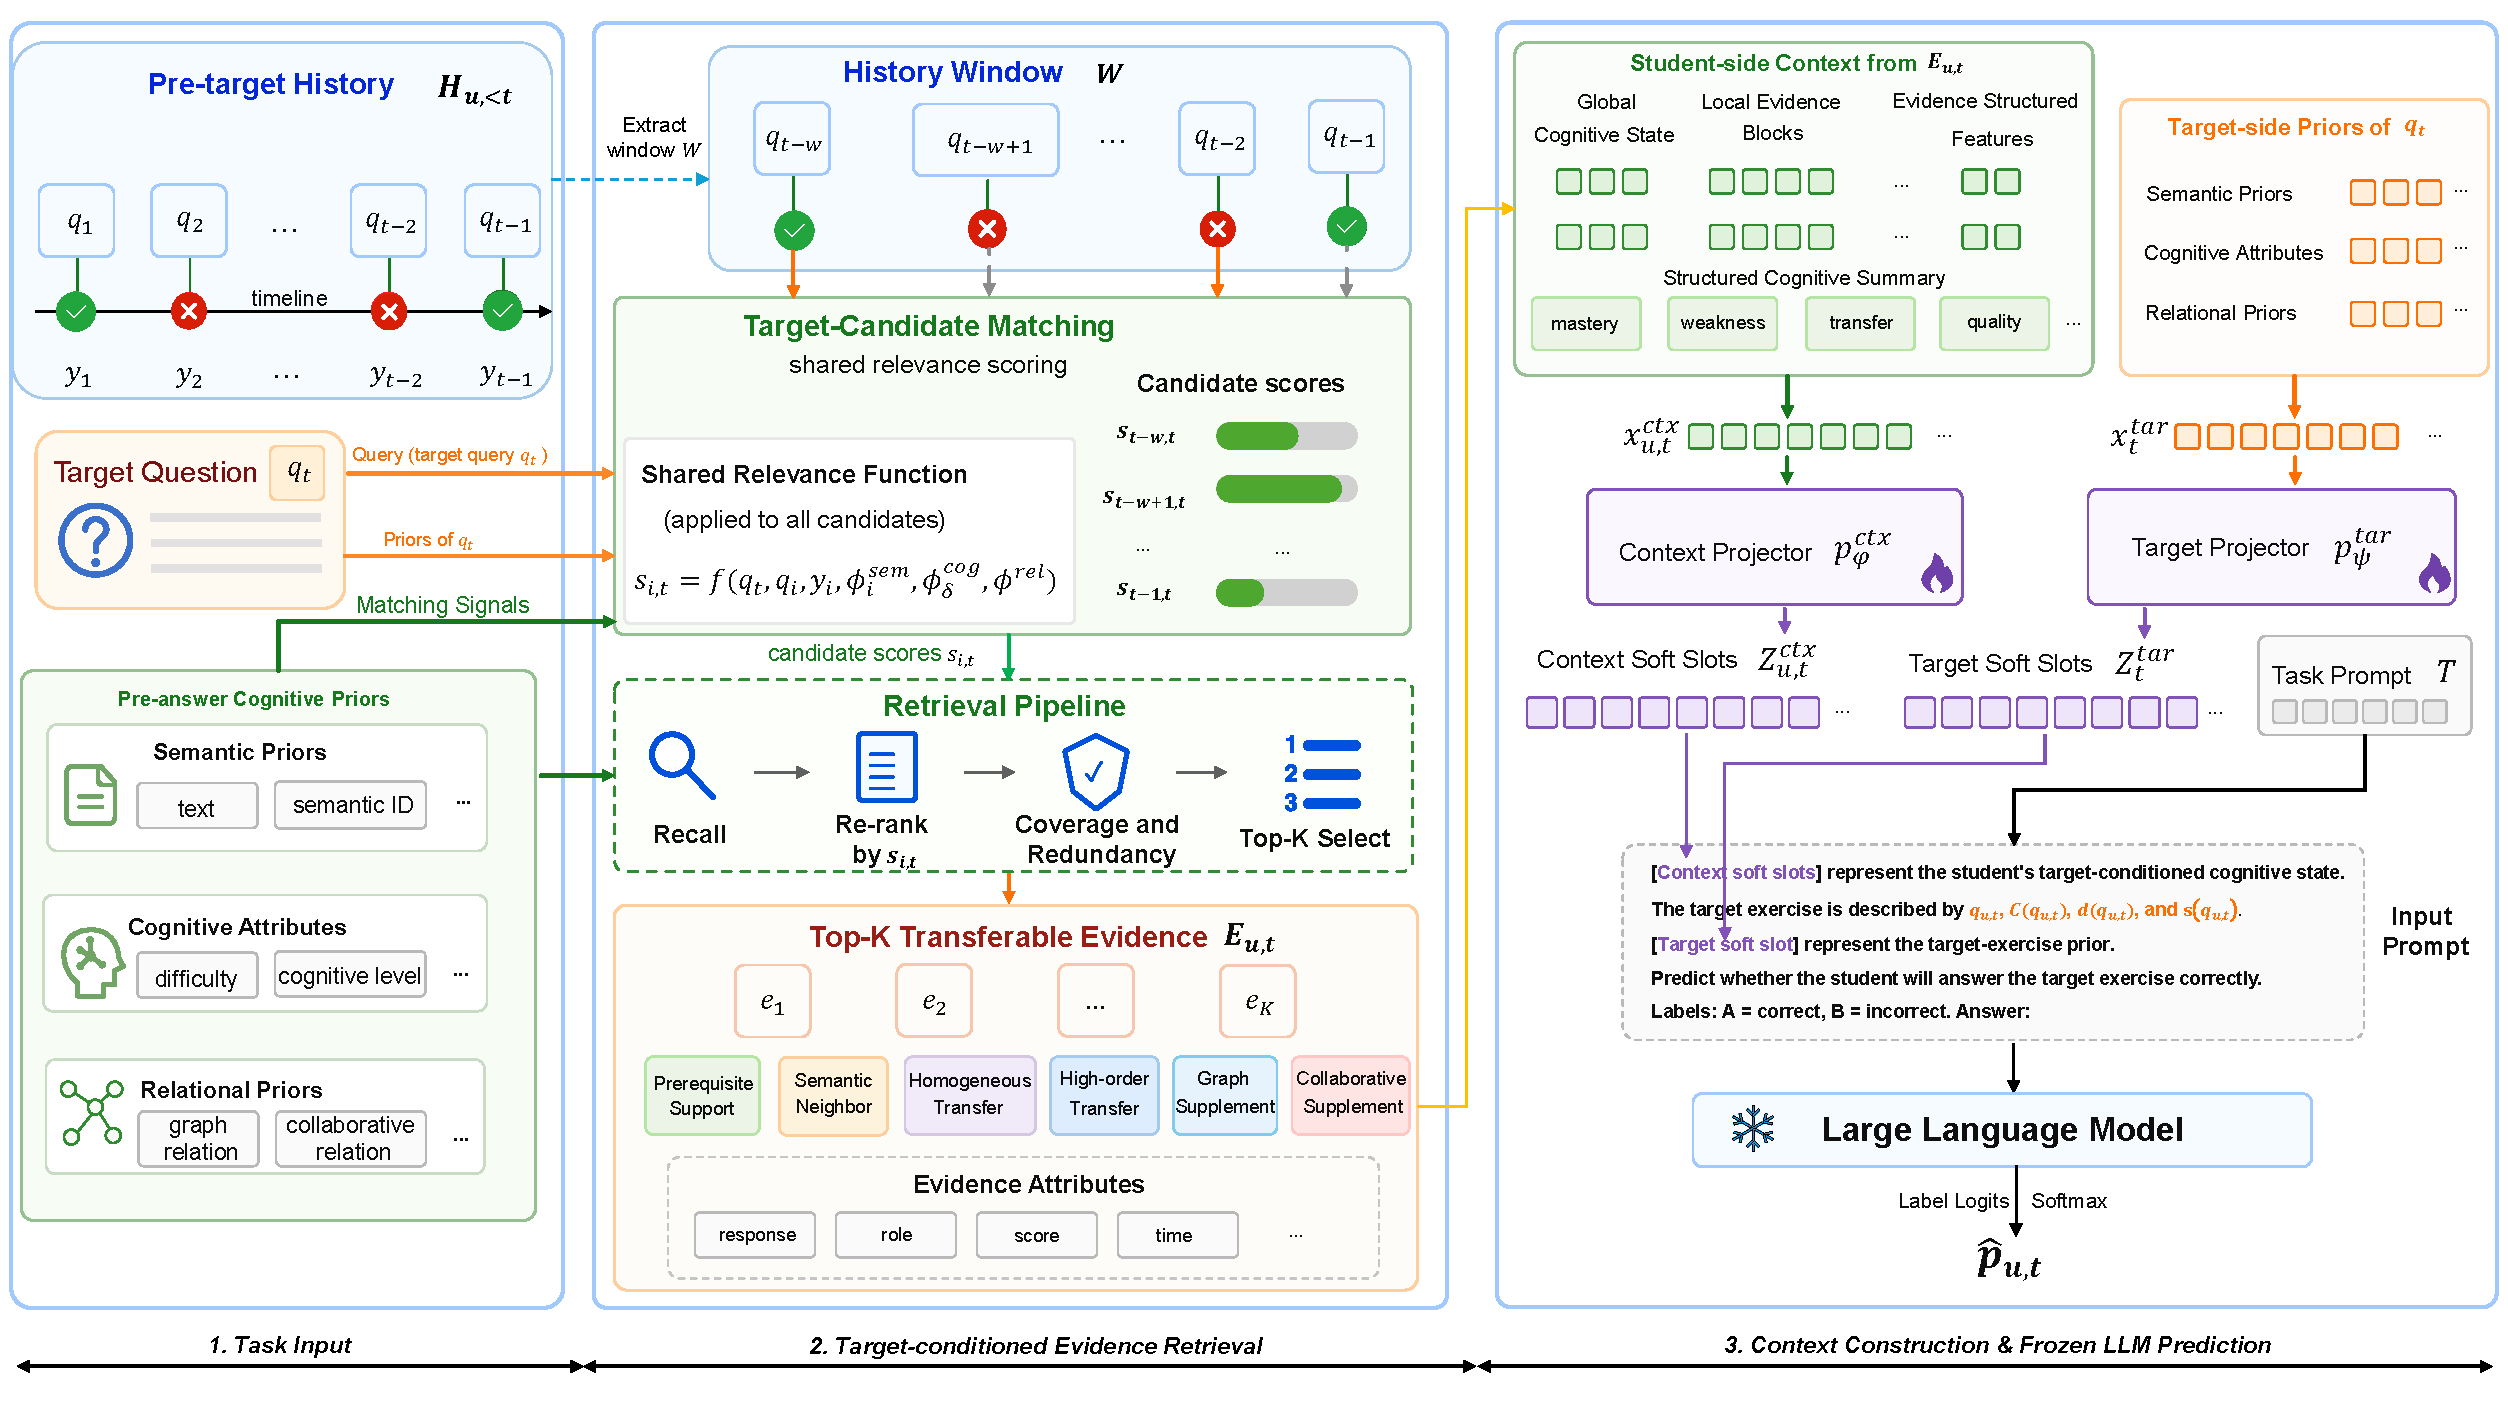
\includegraphics[width=\linewidth]{figures/model.pdf}
\caption{Overview of Cognitive-RAG KT. (a) Target-conditioned retrieval recalls historical interactions using multiple relations and selects up to $K$ complementary evidence interactions through reranking and greedy selection. (b) Evidence records and a schema-constrained summary are jointly encoded and concatenated with summary and state features. The resulting context and target-question representation are mapped into continuous soft slots to condition a frozen LLM for response prediction.}
\label{fig:cognitive-rag-overview}
\end{figure}

\subsection{Question Representation}

For each question \(q\), we construct text, hierarchical semantic, semantic, and collaborative representations. The hierarchical semantic representation encodes representative words from coarse- and fine-grained clusters. The semantic representation fuses text and hierarchical semantics and adjusts the result using cognitive-level information and Rasch difficulty. The four representations are used in historical interaction retrieval and question context construction.

\paragraph{Text and Hierarchical Semantic Representations.}

Let \(x_q\) denote the textual content of question \(q\). A fixed pretrained text encoder maps \(x_q\) to \(\mathbf{h}_q^{\mathrm{text}}\).

\textit{Hierarchical semantics extraction.}

We apply two-level clustering to the text representations of training questions. The first level forms coarse-grained clusters, and the second partitions each coarse-grained cluster into fine-grained clusters.

\textit{Hierarchical semantics translation.}

We describe each question's cluster assignments using representative words: the most frequent word from its coarse-grained cluster and up to two frequent valid words from its fine-grained cluster. These words provide general and specific semantic descriptions, respectively. The resulting word sequence is encoded by the same text encoder to obtain $\mathbf h_q^{\mathrm{hier}}$.

\paragraph{Semantic Representation.}

The text representation and the hierarchical semantic representation are concatenated and mapped through an MLP to obtain \(\mathbf{e}_q= \operatorname{MLP}( [\mathbf{h}_q^{\mathrm{text}}; \mathbf{h}_q^{\mathrm{hier}}])\).

For each concept \(c\), let \(\mathcal{Q}_c\) denote its associated questions. We apply PCA to the representations \(\{\mathbf{e}_q\mid q\in\mathcal{Q}_c\}\) and take the first principal component as the concept direction. We orient this direction using the cognitive-level annotations of these questions, so that larger projections correspond to higher cognitive levels. The resulting unit vector is denoted by \(\mathbf{d}_c\).

For a question associated with multiple concepts, the corresponding concept directions are averaged and normalized to obtain \(\mathbf{d}_q\). The Rasch model provides the question-difficulty parameter \(b_q\)~\cite{rasch1960}, which is mapped to the bounded coefficient \(\mu_q=\tanh(a b_q)\). The semantic representation of question \(q\) is defined as

\begin{equation}
\mathbf{h}_q^{\mathrm{sem}}
=
\mathbf{e}_q+\mu_q\mathbf{d}_q.
\end{equation}

Here, \(\mathbf{d}_q\) determines the direction of the adjustment, while \(\mu_q\) determines its signed magnitude. We aggregate only available concept directions; if none is available or their mean has zero norm, we set $\mathbf d_q=\mathbf0$, yielding $\mathbf h_q^{\mathrm{sem}}=\mathbf e_q$.

\paragraph{Collaborative Representation.}

We train a skip-gram Word2Vec model on chronologically ordered question sequences constructed from training interactions. The learned embedding $\mathbf h_q^{\mathrm{col}}$ captures which questions tend to appear near question $q$ in these sequences.

\paragraph{Final Question Representation.}

The four representations are concatenated as

\begin{equation}
\mathbf{z}_q
=
\left[
\mathbf{h}_q^{\mathrm{text}};
\mathbf{h}_q^{\mathrm{hier}};
\mathbf{h}_q^{\mathrm{sem}};
\mathbf{h}_q^{\mathrm{col}}
\right].
\end{equation}

For the target question \(q_t\), \(\mathbf{z}_{q_t}\) is used for prediction.

\subsection{Historical Interaction Retrieval}

Given the student interaction history \(\mathcal{H}_t\) and the target question \(q_t\), the retrieval module first recalls potentially relevant historical interactions and then selects a compact evidence set. The resulting evidence set \(E_t\) is used to construct the historical evidence context for predicting the response to \(q_t\).

\paragraph{Candidate Recall.}

For each admissible interaction, write $h_i=(q_i,y_i)$, $\mathcal C_i=\mathcal C(q_i)$, and $\mathcal C_t=\mathcal C(q_t)$. For each historical interaction \((q_i,y_i)\in\mathcal{H}_t\), we compute a recall score according to its relation to the target question \(q_t\) and its position in the interaction history. The relation is evaluated using concept similarity, cognitive levels, graph relations, and collaborative similarity.

The graph contribution $G_{i,t}$ captures structural connections beyond direct concept overlap. It is the maximum weighted prerequisite or neighbor match over concept pairs from $\mathcal C_i$ and $\mathcal C_t$, with zero assigned when no match exists. This contribution allows historical questions involving related concepts to support target prediction.

Let $J_{i,t}$ be the Jaccard similarity between $\mathcal C_i$ and $\mathcal C_t$. Define the cognitive-level difference as $\Delta\ell_{i,t}=\ell_{q_t}-\ell_{q_i}$ and the semantic similarity as $s_{i,t}=\cos(\mathbf h_{q_i}^{\mathrm{sem}},\mathbf h_{q_t}^{\mathrm{sem}})$. For a lower-level historical question, we combine its observed response with a diagnostic probability:

\begin{equation}
M_{i,t}
=
\rho y_i+(1-\rho)p_{i\mid t}^{\mathrm{diag}},
\end{equation}

where $p_{i\mid t}^{\mathrm{diag}}$ estimates the probability of answering $q_i$ correctly under a target-conditioned student state constructed from recent admissible interactions, and $\rho$ controls the balance between the observed response and the diagnostic estimate. The cognitive contribution is

\begin{equation}
\begin{aligned}
L_{i,t}
&=
\begin{cases}
w_{\mathrm{pre}}J_{i,t}M_{i,t}
e^{-\gamma_{\mathrm{pre}}\Delta\ell_{i,t}},
& \Delta\ell_{i,t}>0,\\
w_{\mathrm{peer}}s_{i,t},
& \Delta\ell_{i,t}=0,\ J_{i,t}+G_{i,t}>0,\\
w_{\mathrm{semantic}}s_{i,t},
& \Delta\ell_{i,t}=0,\ J_{i,t}+G_{i,t}=0,\\
w_{\mathrm{high}}J_{i,t}
[\beta_+y_i-\beta_-(1-y_i)]
e^{-\gamma_{\mathrm{high}}|\Delta\ell_{i,t}|},
& \Delta\ell_{i,t}<0.
\end{cases}
\end{aligned}
\end{equation}

The branch weights control the contributions of different cognitive relations. The $\gamma$ coefficients govern attenuation with cognitive-level distance, and $\beta_+$ and $\beta_-$ weight correct and incorrect higher-level responses, respectively. For questions at the same cognitive level, an explicit concept or graph match defines the peer relation; otherwise, semantic similarity defines the semantic relation.

Collaborative similarity provides an additional relation derived from the collaborative representations of \(q_i\) and \(q_t\). It is downweighted when the concept, cognitive level, and graph relations already provide strong evidence. The resulting collaborative score is denoted by \(C_{i,t}\).

The four relations are combined as

\begin{equation}
B_{i,t}=w_JJ_{i,t}+L_{i,t}+w_{\mathrm{graph}}G_{i,t}+w_{\mathrm{col}}C_{i,t},
\end{equation}

where \(L_{i,t}\) includes the weight for the cognitive level relation. The remaining coefficients weight concept similarity, graph relations, and collaborative similarity.

We further account for the cumulative semantic difference between the historical interaction and the target position:

\begin{equation}
D_{i,t}=1+\sum_{\substack{i<j<t\\(q_j,y_j)\in\mathcal H_t}}
\left[1-\operatorname{sim}\left(\mathbf h_{q_j}^{\mathrm{sem}},\mathbf h_{q_t}^{\mathrm{sem}}\right)\right].
\end{equation}

Here, $\operatorname{sim}(\cdot,\cdot)$ denotes cosine similarity. The sum includes only admissible historical interactions between $q_i$ and $q_t$. A larger $D_{i,t}$ indicates greater cumulative semantic difference from the target question.

The final recall score is

\begin{equation}
R_{i,t}=\exp\left(-\alpha D_{i,t}\right)B_{i,t},
\end{equation}

where \(\alpha\) controls the effect of cumulative semantic difference on the recall score. The \(K_1\) historical interactions with the highest recall scores form the candidate set \(\mathcal{A}_t\).

\paragraph{Evidence Selection.}

Candidate recall reduces the interaction history to a candidate set \(\mathcal{A}_t\). Selecting only the highest scoring candidates may retain interactions that cover the same concepts or share the same relation to the target. We therefore select evidence according to target relevance, coverage of concepts or relations absent from the selected set, and similarity to interactions already selected.

For each recalled candidate, selection uses the relation score $B_{i,t}$ without semantic decay and adds a reranker contribution:

\begin{equation}
U_{i,t}=B_{i,t}+w_{\mathrm{rr}}r_{i,t}^{\mathrm{rr}},
\end{equation}

where $r_{i,t}^{\mathrm{rr}}$ is the relevance probability obtained from the reranker's yes/no label logits.

Let $\mathcal S\subseteq\mathcal A_t$ denote the evidence selected so far. Candidate recall retains up to $K_1$ interactions. Evidence selection constructs a final set with a budget of $K_2=K\leq K_1$ interactions. The actual number selected for target $q_t$ is $K_t=\min(K,|\mathcal A_t|)$. 

To construct complementary evidence, we reward newly covered relations and concepts while penalizing similarity to selected interactions. We distinguish six target-conditioned relation roles: prerequisite-level, peer-level, semantic, higher-level, graph, and collaborative. They are denoted by $\mathrm{pre}$, $\mathrm{peer}$, $\mathrm{semantic}$, $\mathrm{high}$, $\mathrm{graph}$, and $\mathrm{collab}$, respectively. The active branch of $L_{i,t}$ supplies the corresponding cognitive-role score, while inactive cognitive roles receive zero. The graph and collaborative role scores are $S_{i,t}^{\mathrm{graph}}=G_{i,t}$ and $S_{i,t}^{\mathrm{collab}}=C_{i,t}$. Let $\mathcal R_i=\{r:S_{i,t}^r>\tau_r\}$ denote the active relation roles of $h_i$ with respect to $q_t$, where $\tau_r$ is the activation threshold for role $r$. 

Define $\mathcal O_i=\mathcal C_i\cap\mathcal C_t$ and $\mathcal V_i=\mathcal N(q_i)\cap\mathcal N(q_t)$, where $\mathcal N(q)$ is the stored set of neighboring concepts. For selected evidence $\mathcal S$, let $\mathcal R_{\mathcal S}$, $\mathcal O_{\mathcal S}$, and $\mathcal V_{\mathcal S}$ denote the corresponding unions. Coverage gain is

\begin{equation}
\begin{aligned}
\operatorname{Cov}(h_i\mid\mathcal S)
={}&|\mathcal R_i\setminus\mathcal R_{\mathcal S}|\\
&+\frac{|\mathcal O_i\setminus\mathcal O_{\mathcal S}|}{|\mathcal C_t|+\varepsilon}
+\frac{|\mathcal V_i\setminus\mathcal V_{\mathcal S}|}{|\mathcal N(q_t)|+\varepsilon},
\end{aligned}
\end{equation}

where $\varepsilon>0$ ensures numerical stability. Redundancy combines concept overlap, overlap between target-conditioned relation roles, and semantic similarity:

\begin{equation}
\operatorname{Red}(h_i,\mathcal S)
=\max\left(\{0\}\cup
\{0.4J_{i,j}+0.2J^{\mathcal R}_{i,j}+0.4s_{i,j}:h_j\in\mathcal S\}\right),
\end{equation}

where $J_{i,j}$ is concept Jaccard similarity, $J^{\mathcal R}_{i,j}=|\mathcal R_i\cap\mathcal R_j|/(|\mathcal R_i\cup\mathcal R_j|+\varepsilon)$, and $s_{i,j}$ is semantic cosine similarity. Thus, a candidate is penalized according to its strongest similarity to existing evidence.

The selection score combines target relevance, coverage gain, and redundancy:

\begin{equation}
F(h_i\mid\mathcal S)
=
U_{i,t}
+\lambda_{\mathrm{cov}}\operatorname{Cov}(h_i\mid\mathcal S)
-\lambda_{\mathrm{red}}\operatorname{Red}(h_i,\mathcal S),
\end{equation}

where $\lambda_{\mathrm{cov}}$ and $\lambda_{\mathrm{red}}$ control the coverage reward and redundancy penalty, respectively.

We initialize the evidence set with the interaction most relevant to the target:

\begin{equation}
h^{(1)} = \operatorname*{\arg\max}_{h_i\in\mathcal{A}_t} U_{i,t}.
\end{equation}

At each subsequent step \(k=2,\ldots,K_t\), we select the candidate with the highest \(F(h_i\mid\mathcal S_{k-1})\). This score rewards target relevance and additional coverage while penalizing redundancy with the selected evidence:

\begin{equation}
h^{(k)}=\operatorname*{\arg\max}_{h_i\in \mathcal{A}_t\setminus\mathcal{S}_{k-1}} F(h_i\mid\mathcal{S}_{k-1}),
\qquad 
\mathcal{S}_{k}=\mathcal{S}_{k-1}\cup\{h^{(k)}\},
\end{equation}

where $\mathcal S_1=\{h^{(1)}\}$. After \(K_t\) interactions have been selected, the final evidence set is

\begin{equation}
E_t=\mathcal{S}_{K_t}.
\end{equation}

\subsection{Context Construction}

Each selected interaction is represented by its question text, observed response, relation role, overlapping concepts, cognitive-level difference, and selection support score. The support score is the score used at the step when the interaction was selected. We serialize these records in greedy selection order to form the evidence text $T_t^{\mathrm{evidence}}$.

A schema-constrained summary provides a compact account of the selected evidence, including mastered and weak concepts, transfer state, response risk, evidence quality, and a concise diagnosis. The summary generator receives target information, serialized evidence attributes, and a performance summary. The performance summary is computed from the selected evidence and the dynamic student prior. We jointly encode the rendered summary $T_t^{\mathrm{summary}}$ and evidence text, then concatenate the encoding with summary features $\mathbf f_t$ and state features $\mathbf n_t$:

\begin{equation}
x_t^{\mathrm{hist}}
=
[\operatorname{Enc}(T_t^{\mathrm{summary}}\Vert T_t^{\mathrm{evidence}});
\mathbf f_t;\mathbf n_t],
\qquad
x_t^{\mathrm{ques}}=\mathbf z_{q_t}.
\end{equation}

Here, $\operatorname{Enc}$ denotes a frozen pretrained text encoder, $\Vert$ denotes text concatenation, and semicolons denote feature-vector concatenation. The summary features $\mathbf f_t$ are derived from concept counts, concept-presence indicators, diagnosis length, risk, and evidence quality. The state features $\mathbf n_t$ contain the dynamic student prior and normalized candidate and evidence counts. Target text, concept annotations, and cognitive level also provide textual information in the prediction prompt. The historical and target contexts jointly condition the response predictor.

\subsection{LLM Response Prediction}

The prediction module maps the historical context \(x_t^{\mathrm{hist}}\) and the question context \(x_t^{\mathrm{ques}}\) into the token embedding space of the frozen LLM. The LLM then estimates the probability of a correct response from the logits of two candidate labels.

\paragraph{Context Projection.}

Two projection networks map the historical and question contexts into the frozen LLM's token embedding space:

\begin{equation}
\mathbf{Z}_t^{\mathrm{hist}}=P_{\phi}^{\mathrm{hist}}\left(x_t^{\mathrm{hist}}\right),\qquad
\mathbf{Z}_t^{\mathrm{ques}}=P_{\psi}^{\mathrm{ques}}\left(x_t^{\mathrm{ques}}\right),
\end{equation}

where \(\mathbf{Z}_t^{\mathrm{hist}}\) and \(\mathbf{Z}_t^{\mathrm{ques}}\) are sequences of continuous embeddings compatible with the token embedding dimension of the LLM.

The historical context embeddings represent the selected evidence, its attributes, and the schema-constrained summary. The question embeddings represent the current target question. Both groups are incorporated into a fixed knowledge tracing prompt to condition response prediction.

\paragraph{Label-Logit Prediction.}

The prompt defines the knowledge tracing task and two candidate labels for correct and incorrect responses. Given the prompt and the two groups of continuous embeddings, the LLM produces a logit for each label.

Let \(o_t^{+}\) and \(o_t^{-}\) denote the logits assigned to the correct and incorrect labels, respectively. The predicted probability of a correct response is computed as

\begin{equation}
\hat{p}_t=\frac{\exp(o_t^{+})}{\exp(o_t^{+})+\exp(o_t^{-})}.
\end{equation}

Given the observed response \(y_t\in\{0,1\}\), the prediction loss is defined as

\begin{equation}
\mathcal{L}_{\mathrm{pred}}=-\sum_t\left[y_t\log\hat{p}_t+(1-y_t)\log(1-\hat{p}_t)\right].
\end{equation}

Before response-prediction training, we train the question-representation MLP and the model producing the dynamic diagnostic prior, then fix their parameters. Response-prediction training updates only the historical-context and question-context projectors. The precomputed feature generators and the prediction LLM also remain fixed.

\section{Experimental Setup}

We evaluate Cognitive-RAG KT on response prediction for questions involving new KCs, compare it with standard KT models, and examine the contributions of retrieval and evidence construction.

\subsection{Datasets and Evaluation Protocol}

We use three public KT datasets: FoundationalASSIST \cite{worden2026foundationalassist}, XES3G5M \cite{liu2023xes3g5m}, and MOOCRadar \cite{yu2023moocradar}. Each dataset contains chronologically ordered student--question interactions with binary response outcomes and question--concept annotations. Table~\ref{tab:dataset‑split‑statistics} summarizes the datasets before evaluation targets are constructed.

\begingroup
\setlength{\intextsep}{6pt}

\begin{table}[H]
\centering
\small
\setlength{\tabcolsep}{4pt}
\renewcommand{\arraystretch}{1.1}
\caption{Statistics of the three datasets before target construction.}
\label{tab:dataset‑split‑statistics}
\begin{tabular*}{\linewidth}{@{\extracolsep{\fill}}lrrrr@{}}
\toprule
\textbf{Dataset} & \textbf{Students} & \textbf{Questions} & \textbf{Concepts} & \textbf{Interactions} \\
\midrule
FoundationalASSIST & 5,000 & 2,492 & 143 & 999,467 \\
XES3G5M & 4,833 & 3,903 & 575 & 609,867 \\
MOOCRadar & 14,224 & 9,383 & 9,985 & 898,933 \\
\bottomrule
\end{tabular*}
\end{table}
\endgroup

A question $q_{u,t}$ is included as a test target when $\mathcal{C}(q_{u,t})\cap\mathcal{C}_{\mathrm{ho}}\neq\emptyset$.

For each target, the student history is

\[\mathcal{H}^{\mathrm{tr}}_{u,<t}=\left\{(q_{u,i},y_{u,i})\mid
i<t,\;\mathcal{C}(q_{u,i})\subseteq\mathcal{C}_{\mathrm{tr}}
\right\}.\]

The model uses the questions and observed responses in this history, together with target information such as question text and concept annotations.

We exclude each student's first interaction because it has no preceding history. Table~\ref{tab:cold‑start‑split‑statistics} reports the resulting training and test target counts and concept statistics.

\begin{table}[t]
\centering
\scriptsize
\setlength{\tabcolsep}{3pt}
\caption{Statistics of training and test targets and KCs. Percentages indicate the proportion of new KCs among all KCs appearing in test targets.}
\label{tab:cold‑start‑split‑statistics}
\begin{tabular}{lrrrrr}
\toprule
\textbf{Dataset} & \textbf{Train targets} & \textbf{Test targets} & \textbf{Train KCs} & \textbf{Test KCs} & \textbf{New KCs} \\
\midrule
FoundationalASSIST & 328,433 & 666,034 & 27 & 127 & 113 (89.0\%) \\
XES3G5M & 108,319 & 496,715 & 99 & 524 & 476 (90.8\%) \\
MOOCRadar & 66,512 & 818,197 & 138 & 2,703 & 2,642 (97.7\%) \\
\bottomrule
\end{tabular}
\end{table}

\subsection{Baselines}

We compare Cognitive-RAG KT with twelve KT baselines. DKT~\cite{piech2015deep} uses a recurrent neural network to encode response histories. SAKT~\cite{pandey2019sakt} uses self-attention to relate historical interactions to the target question. SAINT~\cite{choi2020saint} encodes question and response sequences with a Transformer encoder--decoder. AKT~\cite{ghosh2020akt} combines question similarity with context-aware distance and exponential decay in its attention weights. simpleKT~\cite{liu2023simplekt} combines question-specific variations with ordinary dot-product attention.

DIMKT~\cite{shen2022dimkt} incorporates question difficulty into question representations and knowledge-state updates. QIKT~\cite{chen2023qikt} models question-sensitive knowledge acquisition and problem solving and uses an item response theory prediction layer. KeenKT~\cite{li2026keenkt} represents knowledge states with normal inverse Gaussian distributions and uses distribution-based attention to track their evolution.

sparseKT~\cite{huang2023sparsekt} uses sparse attention to retain high-scoring historical interactions. DenoiseKT~\cite{deng2025denoisekt} enhances question representations with a graph neural network and suppresses irrelevant interactions through denoised attention. TCKT~\cite{huang2024tckt} combines causal self-attention with temporal information to model learning and forgetting. RobustKT~\cite{guo2025robustkt} decouples cognitive patterns from random factors in response histories.

Each baseline receives historical question or concept IDs, observed responses, and target IDs through its standard input interface. Cognitive-RAG KT additionally uses question text and collaborative representations, together with retrieved evidence and LLM-generated summaries. All methods use the same data splits, history constraints, and test targets.

\subsection{Implementation Details}

Rasch difficulty, collaborative representations, and graph statistics based on interaction or co-occurrence data are estimated from training interactions and fixed during evaluation. Standardization, clustering, and PCA are also fitted on training data before being applied to test items. A frozen pretrained text encoder processes target question text and public metadata. Missing target features are handled using training-derived priors, OOV or zero representations with missingness indicators, or graph mappings based on an unknown node or public metadata, as appropriate.

We set the final evidence budget to $K=K_2=6$ in the main experiments. In the prediction stage, Qwen3-8B remains frozen and only the historical-context and question-context projection networks are trained. We report AUC, ACC, F1, and RMSE, with AUC as the primary metric.


\section{Results and Analysis}

\subsection{Overall Prediction Performance}

Table~\ref{tab:main-results} shows that Cognitive-RAG KT achieves the highest AUC on all three datasets. Compared with DenoiseKT, the strongest baseline in AUC, it obtains absolute AUC gains of 0.1248, 0.1158, and 0.0587 on FoundationalASSIST, XES3G5M, and MOOCRadar, respectively. These results support the framework's effectiveness for response prediction on questions involving new KCs under the evaluated setting.

\begin{table}[t]
\centering
\scriptsize
\setlength{\tabcolsep}{1.5pt}
\renewcommand{\arraystretch}{1.05}
\caption{Prediction performance on three datasets. The best result is bold, and the best baseline result is underlined.}
\label{tab:main-results}
\begin{tabular}{@{}l*{12}{c}@{}}
\toprule
\multirow{2}{*}{\textbf{Method}}
& \multicolumn{4}{c}{\textbf{FoundationalASSIST}}
& \multicolumn{4}{c}{\textbf{XES3G5M}}
& \multicolumn{4}{c}{\textbf{MOOCRadar}} \\
\cmidrule(lr){2-5}
\cmidrule(lr){6-9}
\cmidrule(lr){10-13}
& AUC & ACC & F1 & RMSE
& AUC & ACC & F1 & RMSE
& AUC & ACC & F1 & RMSE \\
\midrule
DKT & 0.5053 & 0.5053 & 0.5621 & 0.5085 & 0.5006 & 0.5013 & 0.6125 & 0.5100 & 0.4830 & 0.4932 & 0.6062 & 0.5161 \\
SAKT & 0.5974 & 0.5902 & 0.6667 & 0.5396 & 0.5636 & 0.7011 & 0.8127 & 0.4960 & 0.7090 & 0.7779 & 0.8666 & 0.4103 \\
SAINT & 0.6184 & 0.6226 & 0.7144 & 0.4857 & 0.5692 & 0.7831 & \underline{0.8773} & 0.4211 & 0.6637 & 0.7024 & 0.8107 & 0.4476 \\
AKT & 0.6430 & 0.6360 & 0.7195 & 0.4855 & 0.6065 & 0.7503 & 0.8504 & 0.4235 & 0.7357 & 0.8099 & 0.8895 & 0.3716 \\
DIMKT & 0.6250 & 0.6388 & \underline{0.7414} & 0.4839 & 0.5771 & 0.7607 & 0.8601 & 0.4228 & 0.7385 & 0.8345 & 0.9066 & 0.3518 \\
QIKT & 0.6250 & 0.6378 & 0.7377 & 0.4857 & 0.6049 & 0.7712 & 0.8670 & 0.4154 & 0.7806 & 0.8371 & 0.9081 & 0.3444 \\
TCKT & 0.6011 & 0.5967 & 0.6760 & 0.5130 & 0.6004 & 0.7635 & 0.8613 & 0.4193 & 0.7702 & 0.8220 & 0.8965 & 0.3559 \\
SimpleKT & 0.5981 & 0.5625 & 0.6158 & 0.5367 & 0.5726 & 0.7312 & 0.8363 & 0.4431 & 0.7582 & 0.8207 & 0.8953 & 0.3596 \\
SparseKT & 0.6067 & 0.6067 & 0.6918 & 0.5109 & 0.5810 & 0.7338 & 0.8381 & 0.4407 & 0.7387 & 0.8180 & 0.8941 & 0.3668 \\
DenoiseKT & \underline{0.6557} & \underline{0.6469} & 0.7340 & \underline{0.4694} & \underline{0.6384} & \underline{0.7839} & 0.8768 & \underline{0.4028} & \underline{0.7817} & \underline{0.8391} & \underline{0.9094} & \underline{0.3415} \\
RobustKT & 0.6252 & 0.6098 & 0.6835 & 0.4903 & 0.5745 & 0.7413 & 0.8448 & 0.4392 & 0.7448 & 0.8297 & 0.9029 & 0.3555 \\
KeenKT & 0.6246 & 0.6226 & 0.7054 & 0.4824 & 0.6232 & 0.7612 & 0.8577 & 0.4182 & 0.7758 & 0.8067 & 0.8849 & 0.3664 \\
\midrule
\textbf{Cognitive-RAG KT} & \textbf{0.7805} & \textbf{0.7335} & \textbf{0.7998} & \textbf{0.4239} & \textbf{0.7542} & \textbf{0.8046} & \textbf{0.8873} & \textbf{0.3791} & \textbf{0.8404} & \textbf{0.8521} & \textbf{0.9111} & \textbf{0.3322} \\
\bottomrule
\end{tabular}
\end{table}

Cognitive-RAG KT also achieves the highest ACC and F1 and the lowest RMSE on all three datasets. Relative to DenoiseKT, RMSE decreases by 0.0455, 0.0237, and 0.0093 on FoundationalASSIST, XES3G5M, and MOOCRadar, respectively. These gains cover both classification metrics and probability prediction error.

\subsection{Ablation Study}

We evaluate three ablations of retrieval and evidence construction in Table~\ref{tab:component-ablation}. The w/o Retrieval (Recent-$K$) variant replaces target-conditioned selection with the most recent $K$ admissible interactions and generates its summary from this replacement history. The target information, evidence budget, summary-generation procedure, predictor, and training settings remain unchanged. The w/o Summary variant removes the generated summary text and its derived features $\mathbf f_t$ from the historical context. The w/o Fine-Grained Evidence variant replaces the entire historical context $x_t^{\mathrm{hist}}$ with a 12-dimensional vector of coarse numerical features summarizing the student's response history and target position. The replaced context includes the retrieved interaction records, relation attributes, and generated summary. The target-question branch is retained. All variants use the same data splits and evaluation targets.

\begin{table}[t]
\centering
\scriptsize
\setlength{\tabcolsep}{2.5pt}
\caption{Ablation results for retrieval and context construction. Recent-$K$ uses the most recent $K$ admissible interactions. w/o Fine-Grained Evidence replaces the evidence context with coarse numerical features.}
\label{tab:component-ablation}
\begin{tabular}{lccccccccc}
\toprule
\multirow{2}{*}{\textbf{Variant}}
& \multicolumn{3}{c}{\textbf{FoundationalASSIST}}
& \multicolumn{3}{c}{\textbf{XES3G5M}}
& \multicolumn{3}{c}{\textbf{MOOCRadar}} \\
\cmidrule(lr){2-4}
\cmidrule(lr){5-7}
\cmidrule(lr){8-10}
& AUC & ACC & F1
& AUC & ACC & F1
& AUC & ACC & F1 \\
\midrule
Full
& \textbf{0.7805} & \textbf{0.7335} & \textbf{0.7998}
& \textbf{0.7542} & \textbf{0.8046} & \textbf{0.8873}
& \textbf{0.8404} & \textbf{0.8521} & \textbf{0.9111} \\
w/o Retrieval (Recent-$K$)
& 0.7423 & 0.7030 & 0.7728
& 0.7020 & 0.7894 & 0.8791
& 0.7864 & 0.8204 & 0.8958 \\
w/o Summary
& 0.7786 & 0.7240 & 0.7896
& 0.7517 & 0.8014 & 0.8746
& 0.8340 & 0.8439 & 0.9036 \\
w/o Fine-Grained Evidence
& 0.7731 & 0.7280 & 0.7980
& 0.7521 & 0.8030 & 0.8858
& 0.8394 & 0.8439 & 0.9082 \\
\bottomrule
\end{tabular}
\end{table}

Target-conditioned retrieval yields the largest AUC gain in the component comparison. Relative to Recent-$K$, the full model improves AUC by 0.0382, 0.0522, and 0.0540 on FoundationalASSIST, XES3G5M, and MOOCRadar, respectively, and also achieves higher ACC and F1 on each dataset. With the evidence budget and downstream predictor fixed, these gains support target-conditioned history selection over recency-based selection.

The full model also outperforms both w/o Summary and w/o Fine-Grained Evidence on AUC, ACC, and F1 across all three datasets. Removing the summary text and its derived features reduces AUC by 0.0019--0.0064. Compared with w/o Fine-Grained Evidence, the full model improves AUC by 0.0074, 0.0021, and 0.0010 on FoundationalASSIST, XES3G5M, and MOOCRadar, respectively. These comparisons support the complete evidence context, including the summary text and its derived features, for response prediction.

\subsection{Sensitivity to Retrieval Size}

We vary the final evidence budget $K=K_2$ over $\{2,4,6,8,10\}$ on XES3G5M, keeping the candidate recall budget $K_1$ and all other settings fixed. As shown in Figure~\ref{fig:retrieval-size}, AUC and ACC increase and RMSE decreases as $K$ rises from 2 to 6. At $K=6$, AUC reaches 0.7542 and RMSE reaches 0.3791, their best values among the evaluated settings. Increasing $K$ to 8 or 10 does not further improve either metric, although ACC peaks at 0.8051 at $K=8$. With AUC as the primary metric, we use $K=6$ in the main experiments.

\begingroup
\setlength{\intextsep}{4pt}
\setlength{\abovecaptionskip}{4pt}
\setlength{\belowcaptionskip}{0pt}

\begin{figure}[H]
\centering
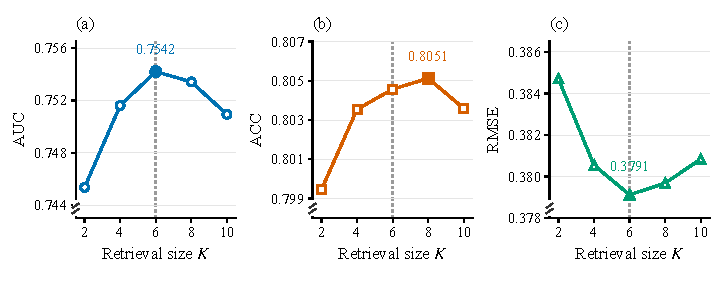
\includegraphics[width=0.90\linewidth]{figures/retrieval_size_sensitivity.pdf}
\caption{Sensitivity to retrieval size on XES3G5M: (a) AUC, (b) ACC, and (c) RMSE. Dashed vertical lines indicate $K=6$, the setting used in the main experiments. Filled markers indicate the best value for each metric. Each panel uses a local vertical-axis range, with a scale-break symbol indicating the omitted interval.}
\label{fig:retrieval-size}
\end{figure}

\endgroup

\clearpage
\subsection{Case Study}

\begingroup
\setlength{\intextsep}{4pt}
\setlength{\abovecaptionskip}{4pt}

\begin{figure}[H]
\centering
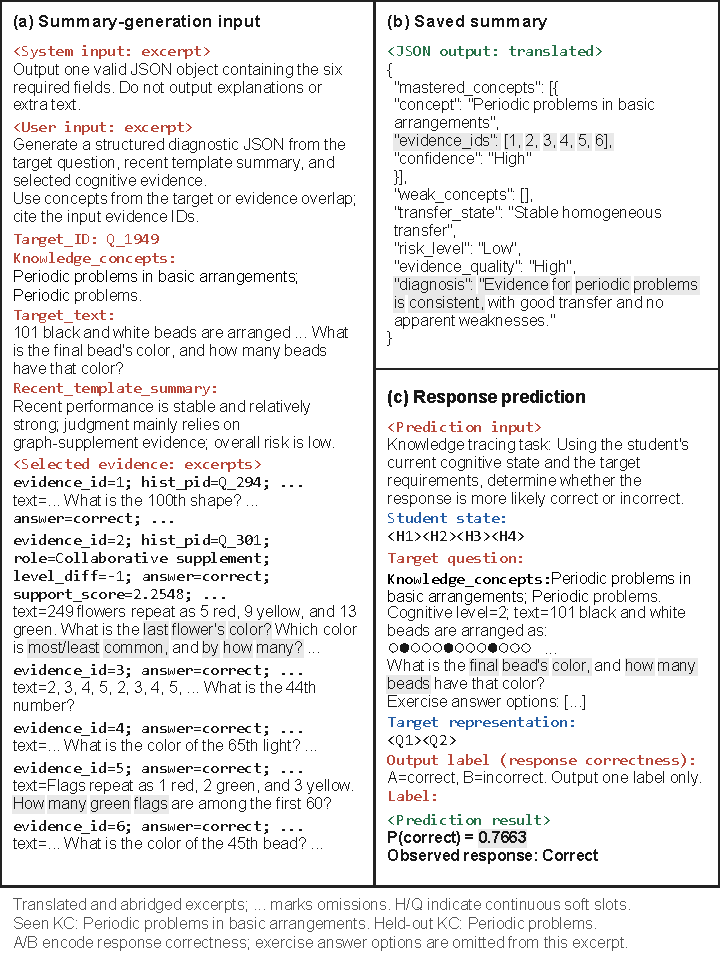
\includegraphics[width=\linewidth]{figures/case_study.pdf}
\caption{Case study of Q\_1949 on XES3G5M. (a) Reconstructed summary-generation input excerpts. (b) The saved structured summary. (c) The prediction prompt and result. Text is translated and abridged; ellipses indicate omissions, and H/Q mark continuous soft-slot positions. Gray highlights identify passages discussed in the text. A/B denote response correctness; exercise answer options are omitted from the displayed excerpt.}
\label{fig:case-study}
\end{figure}
\endgroup

Figure~\ref{fig:case-study} presents a case from XES3G5M for target question Q\_1949. The target involves the training concept ``Periodic problems in basic arrangements'' and the new concept ``Periodic problems''. The question presents a repeating arrangement of 101 beads and asks for the final bead's color and the number of beads of that color.

All six selected historical questions involve the training concept, and the student answered each correctly. E1, E3, E4, and E6 concern identifying elements at specified positions, while E5 concerns counting occurrences. E2 combines final-position identification with quantity comparison and has cognitive level 3, compared with level 2 for the target. Together, these records document correct responses on historical position-finding and counting tasks related to the target.

The saved summary in panel~(b) was generated from the inputs in panel~(a). It cites E1--E6 as evidence for mastery of the shared training concept. It describes the pattern of correct responses on these related questions as ``stable homogeneous transfer''. Panel~(c) shows the prediction prompt, with four history slots H1--H4 before the target question and two target slots Q1--Q2 after it. The correct and incorrect label logits yield a correct-response probability of 0.7663, consistent with the student's observed correct response.

\FloatBarrier

\section{Conclusion}

We propose Cognitive-RAG KT for predicting student responses to questions involving new KCs through target-conditioned evidence retrieval. It combines multiple relations and balances relevance, coverage, and redundancy to select relevant and complementary historical interactions. Structured evidence attributes and a schema-constrained summary organize these interactions into a context representation. This context and the target-question representation condition a frozen language model through soft slots. On three public datasets, the framework outperforms the evaluated standard KT baselines. Component ablations show higher prediction performance with target-conditioned retrieval than with the most recent $K$ admissible interactions. Future work will explore evidence caching and lightweight predictors to improve inference efficiency and support deployment in intelligent tutoring systems.

\bibliographystyle{splncs04}

\bibliography{reference}

\end{document}